\include{template}
\cfoot{} %% if no page number is needed

\begin{document}

\begin{header}
Activité 1 -- Corps purs et mélanges
\end{header}

\section*{Corps purs ou mélanges ?}

Pour chaque élément, dire s'il s'agit d'un corps pur ou d'un mélange.
Justifier votre réponse.

\begin{multicols}{4}
\begin{itemize}
\item[•] eau distillée
\item[•] médicament
\item[•] sirop
\item[•] lingot d'or
\item[•] sel
\item[•] peinture
\item[•] aluminium
\item[•] moutarde
\item[•] air
\item[•] sucre
\end{itemize}
\end{multicols}

\section*{Mélange homogène ou hétérogène ?}

Dire si chaque mélange est homogène ou hétérogène.
Justifier votre réponse.

\begin{center}
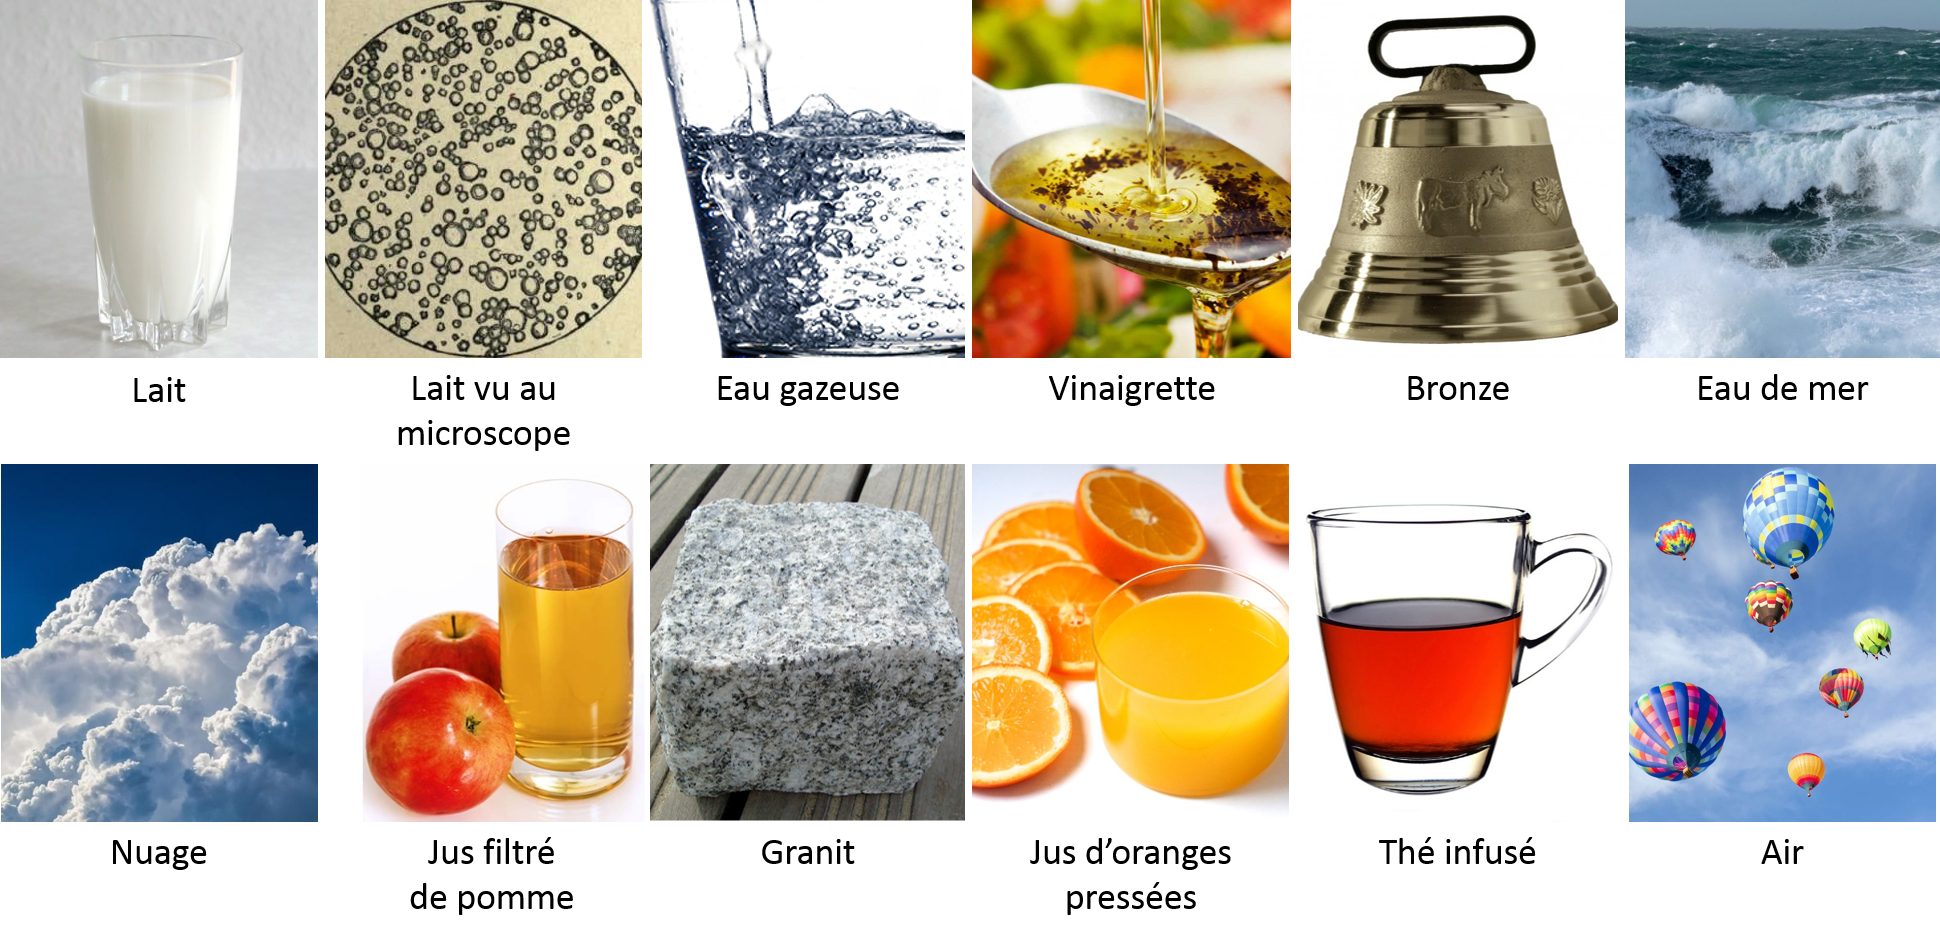
\includegraphics[width=\textwidth]{images/melanges_hom_het.png}
\end{center}

\section*{Composition de l'air}

En s'appuyant sur le texte adapté du site \emph{atmo-france.org}, répondre aux questions suivantes.

\begin{enumerate}
\item Donner la proportion en volume de diazote et de dioxygène dans l'air.
\item Donner le pourcentage volumique de diazote et de dioxygène dans l'air.
\item En moyenne, quel est le volume de dioxygène respiré chaque jour par chacun d'entre nous ?
Exprimer le résultat en $\mathrm{L}$, puis en $\mathrm{m}^3$.
\end{enumerate}

\noindent
\og
\textit{
L'air est un mélange gazeux sans lequel n'existerait pas les conditions nécessaires à la protection et au maintien de la vie : le dioxygène permet la respiration des êtres vivants et le dioxyde de carbone joue un rôle primordial dans le climat de la Terre car il participe à l'effet de serre.
\unit{10}{\liter} d'air contiennent \unit{7{,}8}{\liter} de diazote $\diazote$, \unit{2{,}1}{\liter} de dioxygène $\dioxygene$,  mais également d'autres gaz (gaz rares, dioxyde de carbone $\dioxydedecarbone$, vapeur d'eau $\eau$, etc.).
Instinctivement, chacun respire environ \unit{15000}{\liter} d'air par jour.
}
\fg{}

\end{document}